
为了更好理解用水者对制度变化的响应,本章研究着眼于用水者决策与环境之间的反馈过程进行建模。
在基于主体的模型(Agent-based Model, ABM)中,主体的行为都是在一个由斑块组成的环境中进行的,建模的核心在于设计主体之间的交互规则、主体与环境交互的规则、环境变化的方式。

但在处理实际问题时,我们需要形状不规则的地理空间数据。


\begin{figure}[htb]
    \centering
    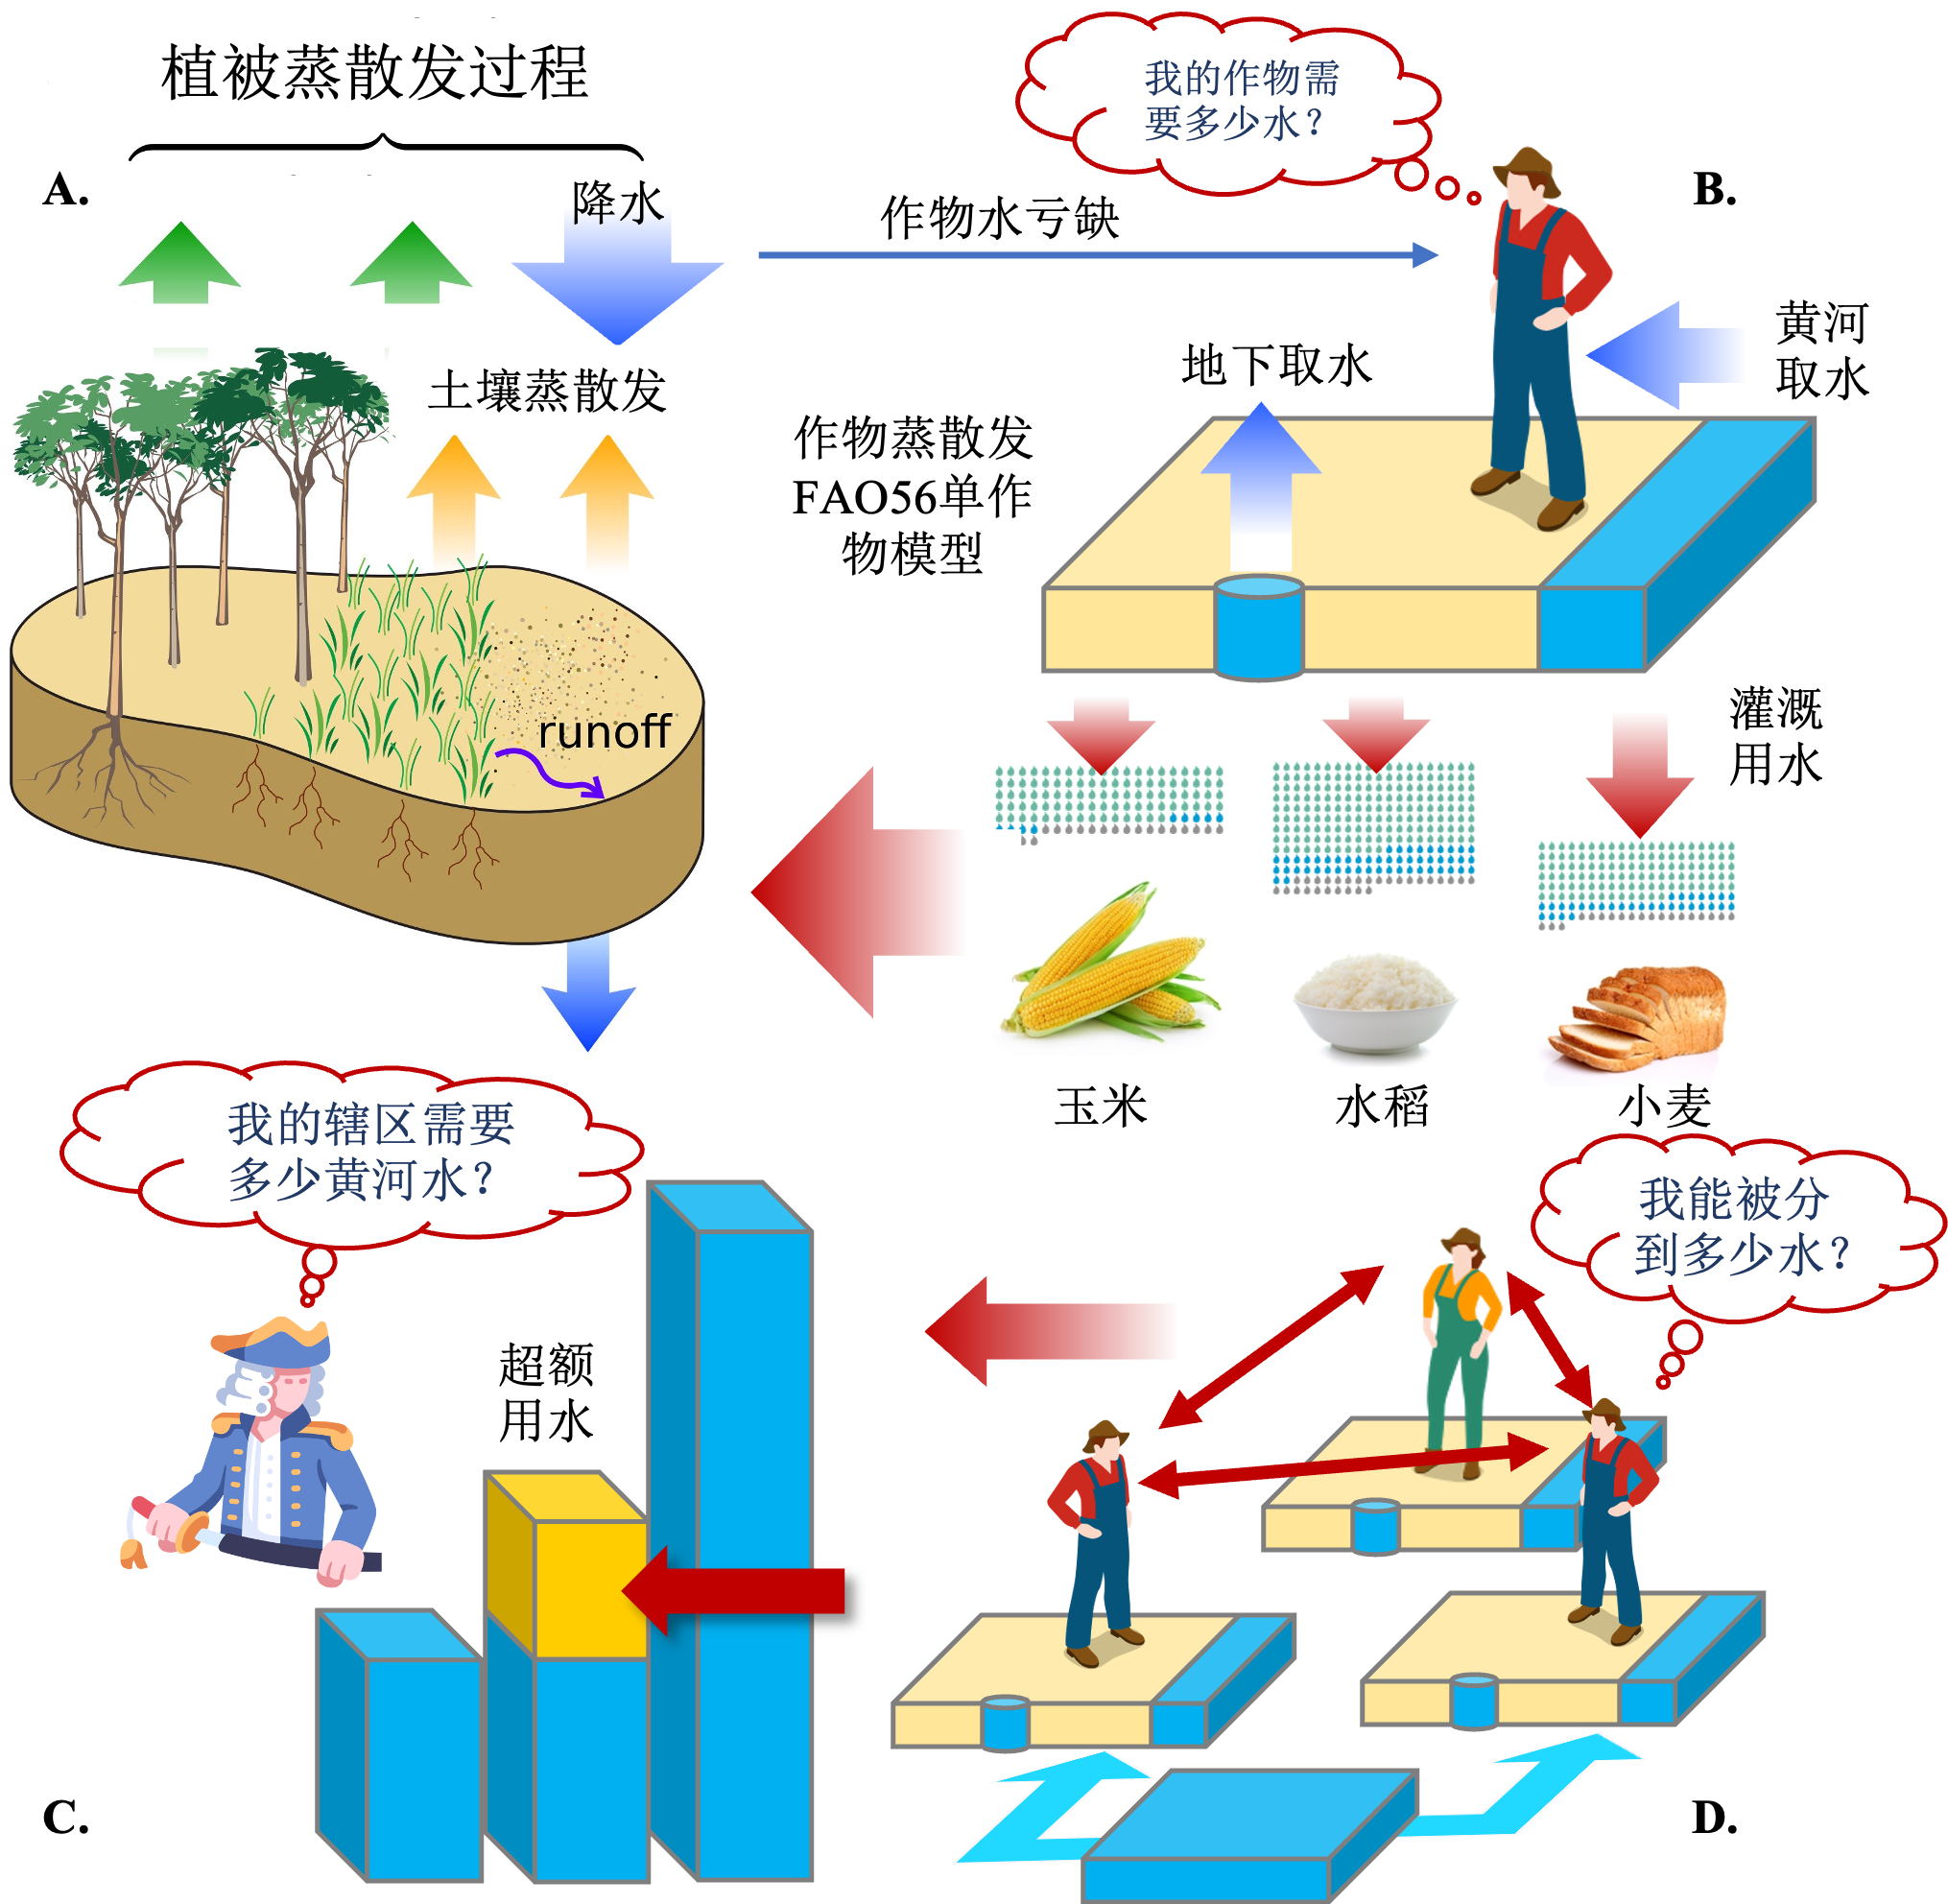
\includegraphics[width=\textwidth]{img/ch6/ch6_framework.png}
    \caption{多主体模型设计框架}\label{ch6:fig:framework}
\end{figure}

\subsubsection*{个体尺度}

水亏缺是考虑灌溉损失后的作物蒸散发与实际降水量之间的差,作物蒸散发则采用国际粮农组织(FAO)推荐的单作物系数法进行计算,由潜在蒸散发和作物蒸散发系数计算得到。

\begin{equation}
    \label{ch6:eq:deficits}
    W_{deficits} = \frac{ET_c - P}{k_{loss}}
\end{equation}

\begin{equation}
    \label{ch6:eq:etc}
    ET_c = ET_{0} * Kc
\end{equation}

其中潜在蒸散发和降水根据主体所处的位置直接从自然模块调用相应属性,作物蒸散发系数$Kc$的同样通过查阅采用国际粮农组织($FAO56$)推荐的作物表得到(表\ref{ch6:tab:crops})。


% Table generated by Excel2LaTeX from sheet '作物物候表'
\begin{table}[htbp]
    % \centering
    \caption[黄河流域三种主要粮食作物的物候表]{黄河流域三种主要粮食作物的物候表$^a$}
      \begin{tabularx}{\textwidth}{p{0.8cm} LLLLL p{0.8cm} p{0.8cm} p{0.8cm}}
      \toprule
      作物  & \multicolumn{1}{l}{播种期} & \multicolumn{1}{l}{萌发期} & \multicolumn{1}{l}{生长期} & \multicolumn{1}{l}{中期} & \multicolumn{1}{l}{后期} & \multicolumn{1}{l}{$Kc_{ini}$} & \multicolumn{1}{l}{$Kc_{mid}$} & \multicolumn{1}{l}{$Kc_{end}$} \\
      \midrule
      小麦    & 4月5日  & 4月25日 & 5月20日 & 7月19日 & 8月18日 & 0.15  & 1.15  & 0.30  \\
      水稻    & 4月15日 & 5月15日 & 6月14日 & 7月14日 & 8月13日 & 1.00  & 1.20  & 0.70  \\
      玉米    & 4月19日 & 5月9日  & 6月13日 & 7月23日 & 8月22日 & 0.15  & 1.20  & 0.50  \\
      \bottomrule
    \end{tabularx}\label{ch6:tab:crops}%
    \footnotesize\\
    $a$ 本模型不考虑冬小麦的种植。
\end{table}%


但在农民生产实际中,基本不可能做到完全按照作物的水亏缺决定灌溉量,而是根据经验,既往文献中通常在水亏缺基础上额外使用一个系数$\alpha$表示实际决策中的灌溉量,该系数估计了农民对作物水亏缺的经验认知与节水灌溉的影响,即实际灌溉用水量$WU$可表示为:

\begin{equation}
    \label{ch6:eq:WU}
    WU = W_{deficits} * \alpha
\end{equation}

但在本章研究中,由于时间跨度较长($1980 \sim 2010$),区域灌溉的节水升级改造是响应制度变化的重要措施,系数$\alpha$一定是剧烈变化的。
因此,本章研究根据用水量$WU$的年际统计数据将尺度下降到月尺度,$WU_i$代表农民在作物生长季在第$i$个月的实际的用水需求,而经验系数$\alpha$的值则可以作为反映灌溉节水的指标,则有:

\begin{equation}
    \label{ch6:eq:WUi}
    WU_i = WU * \frac{W_{deficits, i}}{\sum_{i} W_{deficits, i}}
\end{equation}

其中$i$为模型的每个时间步长单位(月),因此在每步模拟中,可将每个灌溉主体的作物生长用水来源$W$分为降水来源$W_p$、地表水来源$W_s$、地下水来源$W_g$三部分,具体用水决策及模型计算顺序如下:
(1)根据降水和作物蒸散感知水亏缺$W_{deficits}$,如果$W_{deficits}=0$,说明降水已经满足了需求,则作物生长水源$W$就完全由降水提供,$W=W_{p}$;
(2)如果降水无法满足作物生长需求,就根据公式\ref{ch6:eq:WUi}评估当月的水需求$WU$,并设定降水来源$W_{p} = P$;
(3)对于需求$WU > 0$,假定农民首先考虑从地表水获得,根据自己的官方配额$Q_{0}$和超采的配额$Q_{1}$决定多取用多少配额$Q = Q_{0} + Q_{1}$,若$Q > WU$,则地表水使用$W_s = WU$,否则$W_s = Q$;
(4)最后估计地表水开采量$W_g$,所有降水和地表水仍不被满足的用水需求都被认为从地下水获取,即$W_g = WU - W_s - W_p$。

\subsubsection*{地区尺度}

黄河流域的配额制度通常仅细致到地级市范围,如何在地区尺度分配该地区的可供分配的水资源配额取决于主体之间的自组织。
本章研究中假设地区尺度完全根据作物的水亏缺$WU_{deficits}$分配灌溉水量,作为完全的“按需分配”,这是节约配额的理论最优(也是理论最公平的)情景,这也意味着现实中的资源供需匹配不会比本章研究的模拟结果更好。
在数学上,假设总地表水配额为$Q_{C}$的地区$C$中包含$n$个主体,则主体$j$的配额$Q_j$为:

\begin{equation}
    \label{ch6:eq:quota}
    Q_j = Q_{C} * \frac{W_{deficits, j}}{\sum_{j \in C} W_{deficits, j}}
\end{equation}

由于第五章中介绍的分水制度差异及其变化,地区$C$的配额并非固定不变的,在$1987 \sim 1998$年间水资源配额存在可浮动的特性,使用$Q_{\min}$和$Q_{\max}$两个属性进行表达,允许用水个体的实际地表取用水在其间浮动。
$Q_{\max}$由黄河流域各省在$1983$年自主上报的水资源配额需求基础上降尺度到地区和月份来估算(详见表\ref{ch5:tab:quota}),代表自主取水时期满足该地区主体用水需求的能力上限,通常这是官方建议配额$Q_{\min}$的近两倍。
因此,关于$Q_j$的判定规则如公式\ref{ch6:eq:which_quota}所示,与模型当前模拟的年份$yr$有关:

\begin{equation}
    \label{ch6:eq:which_quota}
    Q_j =
    \begin{cases}
        Q_{\max} & \text{when } yr < 1987 \\
        Q_{\in} \leq Q_j \leq Q_{\max} & \text{when } 1987 \leq yr \leq 1998 \\
        Q_{\min} & \text{when } yr > 1998
    \end{cases}
\end{equation}

在$1987 \leq yr \leq 1998$时期,每个主体在计算配额$Q$时如果有较大的用水需求,其$Q_{0} = Q_{\min}$会保证被优先满足,因为这是分水方案中明确保证的合法配额。
由于这个配额没有被强制执行,该主体拥有一定的灵活性索取获得超越官方建议配额$Q_{\min}$的额外配额$Q_{1}$,即超出制度规定但不违背需求上限的“违背制度”部分,该部分配额的值与主体的社会属性有关,详见\ref{ch6:sec:society}\refname{ch6:sec:society}模块的介绍。
但$Q = Q_{0} + Q_{1}$不会超过该主体能被分配到的最大合理配额$Q_{\max}$。

\subsubsection*{流域尺度}

在流域尺度,需要决定主体生成的数量、位置、以及相互作用网络。
本章研究的时间精度是月,考虑作物的生长季主要在$4$月到$8$月之间(见表\ref{ch6:tab:crops}),因此根据统计数据中三类主要作物的灌溉面积和模拟的空间精度来估计每个地级市的主体数量。

\begin{equation}
    n_{C} = \sum_{k=R, M, W}\frac{A_{C, k}}{A_{cell}}
\end{equation}

其中$k = R, M, W$分别代表本研究考虑的三种作物:水稻、玉米和小麦,$A_{C, k}$为该种作物在$C$市的灌溉面积,$A_{cell}$则为每个斑块(栅格)代表的面积。
由于各地级市的面积每年都会变化,主体数量也会每年使用新的统计数据来进行更新。
每个栅格只能同时存在一个主体,在保证主体数量与灌溉面积一致的基础上,主体生成的位置是随机的,概率遵循以人口空间分布的加权平均。

主体决策之间会互相影响,每年的主体数量和位置更新后,还需要预设主体之间的交互关系。
以每个主体为一个节点,存在相互影响的主体间存在连边,那么整个流域可形成一个复杂网络,该网络可包括三种潜在连边:
(1)同一地级市的灌溉主体之间
(2)不同地级市的灌溉主体之间
(3)不同省区的灌溉主体间
由于中国农业基本单元的封闭性,本研究假设不同省之间的主体之间不会互相影响(即不会出现跨省互相影响决策的情况),在同一地级市之内和地级市之间的连边遵循具有固定连边概率的ER随机图(Erdős–Rényi random graphs)构建算法(Erdos and Renyi, 1959),即随机图是一个由$C * n$个节点组成的图,其中同一地级市每对节点连接的概率为$p_n$,不同地级市之间则每对节点的连接概率为$p_C$。
因此一旦概率对$p_n$,$p_C$给定,全流域范围内所有灌溉主体之间可能互相影响的网络拓扑关系就被确定了。

\subsection{模型框架介绍}

虽然多主体模型适用于基于规则的模拟,但它通常会过度简化空间信息,从而使模型变得抽象。
针对这个问题,本章研究的模型在基于地理数据的多主体建模框架“ABSESpy”的基础上搭建。
该框架使用真实的地理空间数据集来构建人工社会生态系统,同时充分考虑人类行为因素。
它支持使用地理空间数据,对具有认知、社会影响和反应等行为的主体进行建模,用户可以专注于分别实现人类行为的逻辑和自然过程的仿真,该框架使得两者之间能够轻松地访问和修改变量值。
该框架可以调度任意数量的自然模块和社会模块,并使它们之间松散耦合。

在本章研究中,人类用水模块通过作物种植和地下水开采来改变自然水平衡模块,自然水平衡模块则通过降水、地表蒸散发的变化来影响人类用水模块中的决策。
种植作物将改变地表覆被,影响水平衡

\subsection{人类用水模块}\label{ch6:sec:society}

个体能够利用他们的主观能动性来做出决定,所以微观个体可能会对某些社会生态环境做出不同的反应。然而,在某种文化规范下,一些反应因为符合社会规范而受到奖励,而另一些反应则因为背离社会规范而受到惩罚。这种深刻的影响塑造了它们在资源进化博弈中的社会学习过程。

这个模块提供了一些函数来测量代理如何因为这些对齐/不对齐而保持或失去社会匹配。
这一过程基于多元理性(Plural rationality theory PRA)的社会理论,这是一个理解个人决策与社会规范影响之间关系的经典框架。多元理性方法框架已被应用于解释水治理的成功与失败。  % TODO citation

多元理性理论可以对复杂的政策问题进行了结构化的诊断,已被运用于。
这个框架指出,任何社会领域都由四种生活方式的动态组合和再创造组成,即等级制度、平等主义、个人主义和宿命论。每种生活方式都包括组织社会关系的特定模式,以及相应的文化偏见。这个理论认为,如果人类文化呈现出丰富的多样性,那是因为指数级的文化形式可以从有限的选择中产生出多种组合 [@verweij2015]。

% Cobb-Douglas函数(https://inomics.com/terms/cobb-douglas-production-function-1456726)
社会得分是一个Cobb-Douglas函数,在福利经济学中常用的,例如幸福指数和人类发展指数。
% [Happy Planet Index](https://happyplanetindex.org/) 
% 人类发展指数(http://hdr.undp.org/en)

考虑到人们不愿意主动得罪别人,也不愿意丧失名誉,我们采用的函数形式是:

\begin{equation}
    S = {(grid)}^m * {(1 - group)}^n
    \label{ch6:eq:society}
\end{equation}

其中 $m$ 是一个农民报告邻居违规用水的次数,$n$ 则是他被报告违规用水的次数,因此:

- $grid^m$ 这部分表达的是一个 Agent 得罪人而感到不舒服
- $group^n$ 这部分表达的是一个 Agent 因为违规被周围人指指点点而感到不舒服

这个社会效用函数在过往的研究中也有使用,如 Castilla-Rho et al., (2017, 2019) [@castilla-rho2017, @castilla-rho2019]. 如果没有指定这两个参数,我们将参考 [@castilla-rho2017] 的研究从数据库中直接为这两个参数指定值。
这个社会效用函数的参数(Grid 和 Group)可以用各个地区的文化差异来进行量化:

% ![CleanShot2022-08-15at08.57.49@2x](https://songshgeo-picgo-1302043007.cos.ap-beijing.myqcloud.com/uPic/CleanShot%202022-08-15%20at%2008.57.49@2x.png)

\subsection{自然水平衡模块}

\subsection{数据处理}

作物物候、气象、灌溉强度、灌溉面积、用水配额等

模型能够模拟各省份绿水(降水+土壤水)/蓝水(地表/地下水)的使用情况
